\documentclass{article}
\usepackage{oconnor}
\usepackage{ wasysym }

%% UPDATE these variables:
\renewcommand{\hwnum}{3}
%\renewcommand{\labelitemii}[$\$][]{}
\title{CSCI 446, Project Design 04}
\author{Group 20: Jack Tetrault, John Hultman, Patrick O'Connor}
%%\date{due: 15 January 2021}

\begin{document}

\maketitle

CSCI 446 Artificial Intelligence

Project 04: Reinforcement Learning and the Racetrack Problem

Elements of Design Document
\begin{enumerate}
    \item UML Class Diagram
    \item Textual Explanation of Major Classes in UML Diagram
    \item Major Design Decisions
    \item Experimental Design for Testing Results
\end{enumerate}
% ============================================
% ============================================
\nextprob{UML Class Diagram}

% ============================================

%\paragraph{Not needed for this project}


\begin{figure}
    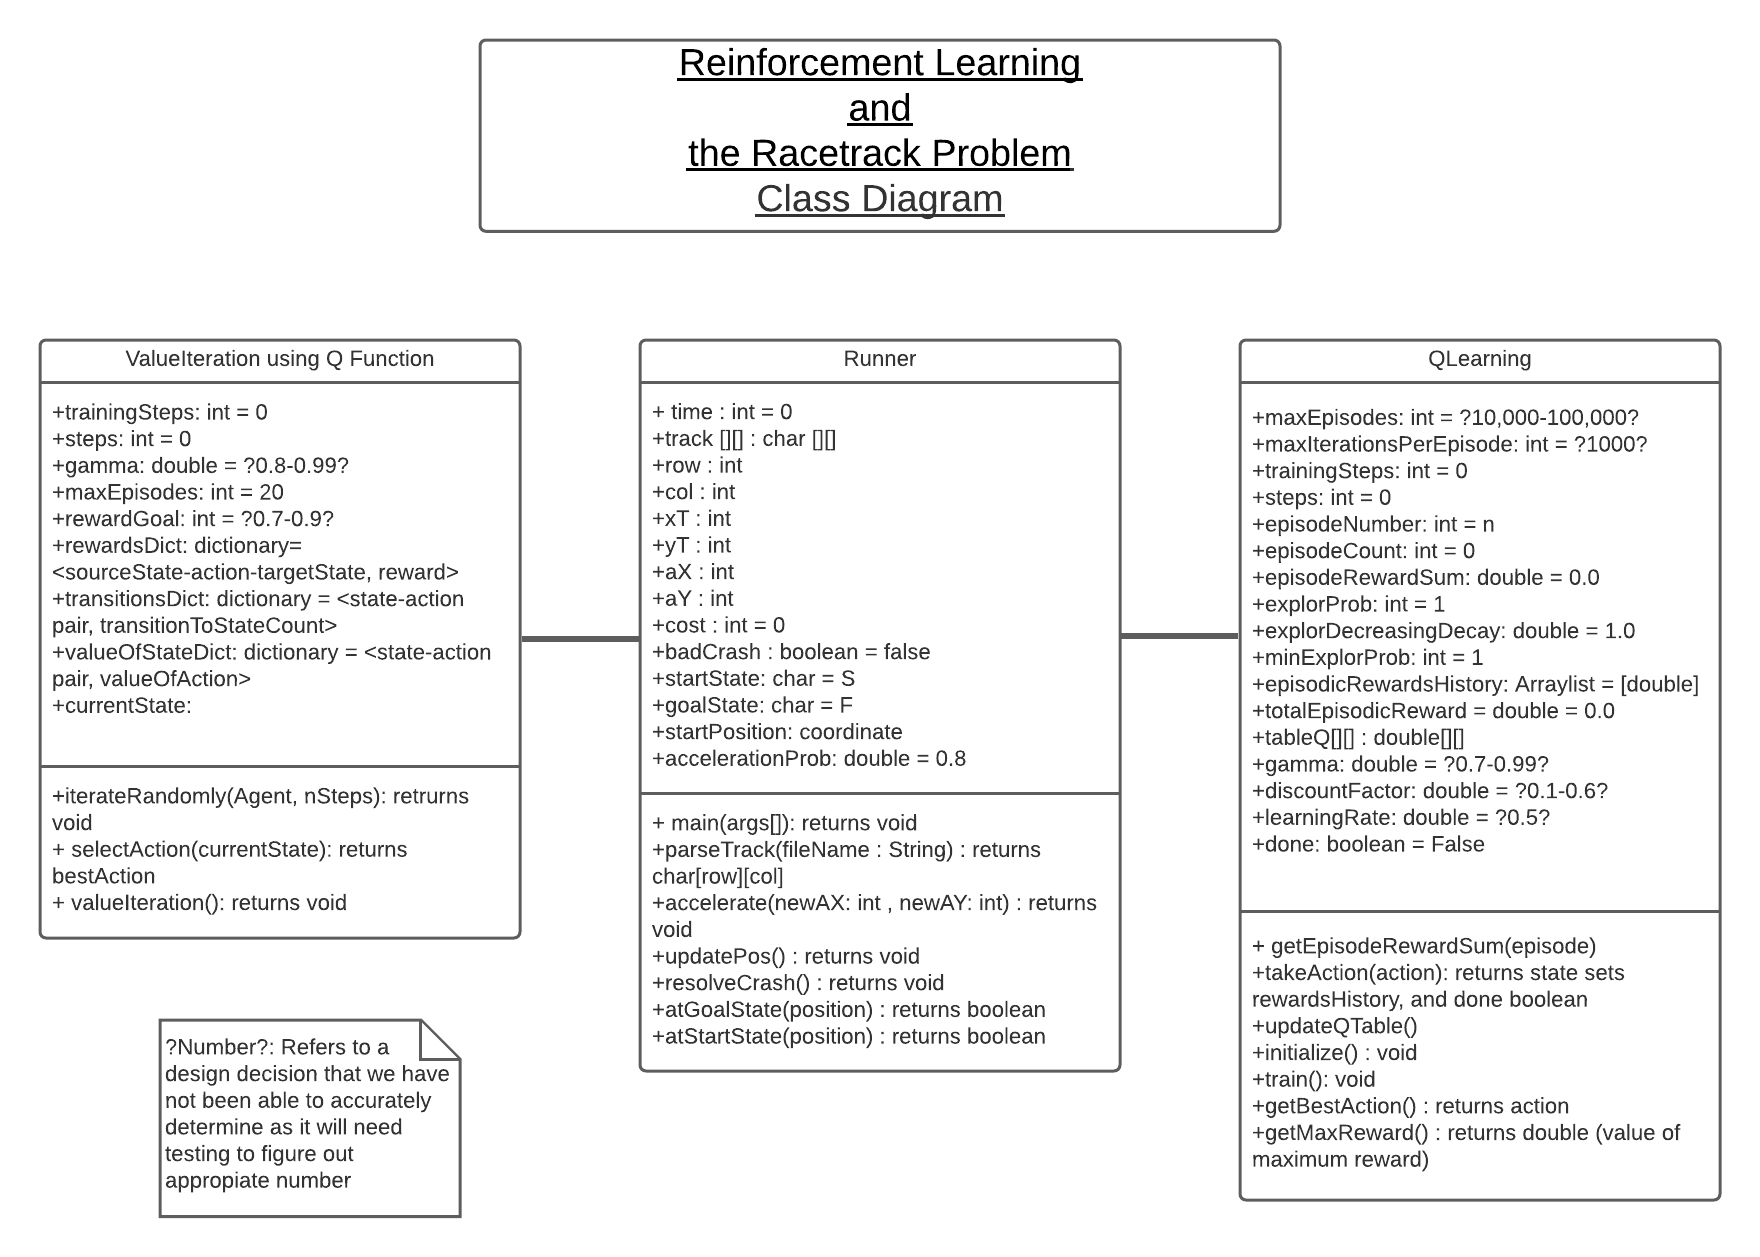
\includegraphics[width=\textwidth]{ReinforcementUMLDiagram.png}
    \caption{UML Drawn using Lucid App}
    \label{fig:num01}
\end{figure}
See figure \ref{fig:num01} for UML Class Diagram

% ============================================
% ============================================
\nextprob{Textual Explanation of Major Classes in UML Diagram}
% ============================================

%Paste paragraphs below here
\begin{enumerate}
    \item Runner Class: This is where the initialization of the track and the learning algorithms will be called from to run. 
    There are several methods we will use in this class to build the game and that the algorithms will use to run on the tracks. 
    main() will be used to drive the entire project. parseTrack() will be used to read in the track file and then it will set the 
    row and col variables while storing the track in a two dimensional array to be used as our track. accelerate(), updatePos(), 
    resolveCrash() will be used in the course of the algorithms running the tracks. atGoalState() and atStartState() will be used to determine 
    if the car has completed the run or not. There are several global variables we will also be using in this class, with the purpose of some 
    being obvious by the names, but xT is the x position at time T, and yT is the y position at time T. aX is the x acceleration and aY is 
    the same but for the y direction which will be updated in accelerate() and this will also increment the cost based on the rules of the 
    game. updatePos() will update xT and yT while checking for collisions or if the car reached the goal state. resolveCrash() will be used 
    to resolve what happens with a crash, if the badCrash flag is enabled then the car will be returned to the start state. 
    \item ValueIteration: The ValueIteration class is the main logic class for implementing the reinforcement learning algorithm value iteration. 
    Within this class we will store a variety of variables but the main data structure that we will use for storing rewards, transitions, 
    and value for state-action pairs will be dictionaries. Within this class there will be functions named iterateRandomly, selectAction, 
    and valueIteration that hold all of our logic. The iterateRandomly will take in agentInfo and a step int of size n. With this 
    information an iteration for nSteps will populate the rewardsDict and transitionDict with random experiences. While iterating we 
    will check to see if we have reached a goalState or if we are at the end of the iteration set. If we reach a goal state a reset 
    of the environment will happen. Else if we reach the end of iteration, the currentState will be set to the newState. 
    The selectAction will be used for analyzing our bestValue and bestAction. This function will begin by initializing bestValue 
    and bestAction to null. From there we will loop through each action available in the current action state. In this loop a value 
    selection will be made from the valueOfStateDict with a key of (state, action). If our bestValue is null or bestValue < the value 
    of the previous selection we will update the bestValue and bestAction appropriately. Once an exhaustive search is completed we 
    will return bestAction. Lastly the logic behind the ValueIteration algorithm will be held in a valueIteration function. In this 
    function a loop of the observable action will be nested in a loop of observedSpace. Within this nested loop, we will initialize 
    the actionValue to 0.0. After this initialization we will create targetValues which will be an accumulation of transitionsDict(state, action). 
    A sum will be collected on this targetValues map. Once a sum has been calculated an iteration on the targetValues items will begin. 
    At each iteration, a key of form state, action, targetState will be grabbed and stored for later use. We will now use the predefined 
    function of selectAction with targetState as the parameter and get our bestAction returned. Using the computed variables create 
    variable tempValue that equals calculatedReward + gamma * VALUEOF(valueOfState(targetState,bestAction). Well add this to the 
    running count of actionValue in an equation of form (item / SUM(transitionsDict(state,action)) * tempValue). From there we'll 
    set ValueOfState(state,action) = actionValue. Once we have hit our rewardGoal the training is complete and we can move forward 
    with testing our model.
    \item QLearning: The QLearning class is the main logic class for implementing the reinforcement learning algorithm Q-Learning. 
    Within this class we will store a variety of variables but the main data structure that we will use for storing complex data 
    like episodic reward history or our Q table will be arrays and multidimensional arrays. To begin this algorithm we will start a 
    loop for a set maxEpisodes count in the range of 10,000 to 100,000. From there we will reset our current state appropriately and 
    our done boolean to false. Nested in the maxEpisode loop we will have another loop that is in range of the maxIterationsPerEpisode 
    which initially we have set to 1000. The next step is deciding whether to explore at random or to explore through the current 
    knowledge base. To complete this we will create a random double that is between 0 and 1, with this we can compare our 
    explorationProbability and decide on the appropriate action. Once an action is decided, the action will be taken through the 
    takeAction(action). This will return the next state, a reward, and the appropriate done boolean. After each action an update 
    on our Q-table will be completed through the updateQTable() and the totalEpisodicReward will be added to. Along with this we 
    will check our done boolean ensuring that we are not at the goal state. If we are not then it is time to update our currentState 
    to the previously taken step. Before continuing in the maxIterationPerEpisode loop the explorationProbability will be decremented 
    appropriately with using the exponential decay formula $y=A_0 e^{kt}$. The last step in this loop is 
    to add our totalEpisodeReward back to our episodicRewardsHistory list. Once our agent has been trained we can use the collected 
    data in this list to determine the performance per n episodes. 
\end{enumerate}



% ============================================
% ============================================
\nextprob{Major Design Decisions}
% ============================================

%Paste paragraphs below here
In this project we have noticed three major design decisions.

We have decided to use the Q function for value iteration reinforcement learning. This is because by implementing this 
strategy, we can get more accurate results by pairing state and actions together, rather than just using the 
state with simple value iteration.

We also decided to implement Q-learning for our second algorithm as opposed to SARSA. This is because we wanted 
to reach an end result matching with the actual optimal policy, rather than resulting in a value that 
matches with a near optimal policy. 

Tunable variables: For our learning rate we will initially set this to a value of 0.5 and tune it up or 
down while staying between 0 and 1 till we find a rate that works well for our testing. We will also set 
our discount factor to somewhere between 0.1 and 0.3 on the “L” and “O” tracks where there is less risk 
if we hit a wall versus a value between 0.3 and 0.6 on the “R” track where crashing into a wall can 
mean being sent back to the start. 




% ============================================
% ============================================
\nextprob{Experimental Design for Testing Results}
% ============================================

%Paste paragraphs below here
Our experimental design for testing our results will consist of us testing the two implemented 
algorithms on three different tracks. Then we will record the number of steps it takes for the car 
to complete a given run and the number of training iterations. We will run this experiment at least 
10 times for each of the three tracks allowing us to come to a more reasonable statistic for each 
algorithm. We will also track the cost for a given run and compare to see which algorithm limits 
the cost more efficiently. We will then represent each algorithm’s run on a given map by plotting 
the number training iterations versus the final cost of each run.

\end{document}

